\section{eo\-Select$<$ EOT $>$ Class Template Reference}
\label{classeo_select}\index{eoSelect@{eoSelect}}
eo\-Select selects a number of individuals from the first argument and puts it in the second.  


{\tt \#include $<$eo\-Select.h$>$}

Inheritance diagram for eo\-Select$<$ EOT $>$::\begin{figure}[H]
\begin{center}
\leavevmode
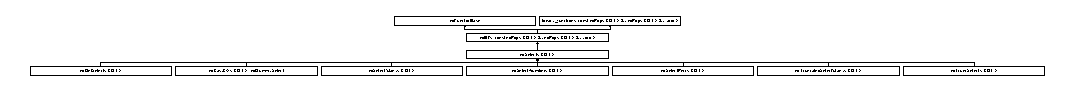
\includegraphics[height=0.786241cm]{classeo_select}
\end{center}
\end{figure}


\subsection{Detailed Description}
\subsubsection*{template$<$class EOT$>$ class eo\-Select$<$ EOT $>$}

eo\-Select selects a number of individuals from the first argument and puts it in the second. 

To emphasize that it should not try to enlarge the population, the second argument is an eo\-Pop\-Range, a simple struct that holds a begin and end iterator to the population 



Definition at line 40 of file eo\-Select.h.

The documentation for this class was generated from the following file:\begin{CompactItemize}
\item 
eo\-Select.h\end{CompactItemize}
